% =============================================================================
% 6. RESULTADOS
% =============================================================================
\section{Resultados}
\label{sec:results}

\subsection{Rendimiento del modelo}

El modelo alcanz\'o un AUC macro de 0.8690 [IC 95\%: 0.8439--0.8931] en el conjunto de validaci\'on oficial, representando una mejora del 8.4\% respecto al baseline con backbone ImageNet (AUC = 0.806). La Tabla~\ref{tab:results-comparison} presenta la comparativa:

\begin{table}[H]
\centering
\caption{Comparativa de rendimiento.}
\label{tab:results-comparison}
\small
\begin{tabular}{lcc}
\toprule
\textbf{Configuraci\'on} & \textbf{AUC} & \textbf{\'Ep.} \\
\midrule
TensorFlow + ImageNet (baseline) & 0.806 & 8 \\
PyTorch + ImageNet & 0.784 & 3 \\
\textbf{PyTorch + XRV (congelado)} & \textbf{0.869} & \textbf{6} \\
Sweep best (lr=0.001) & 0.874 & 5 \\
Fine-tuning (denseblock4) & 0.868 & --- \\
\bottomrule
\end{tabular}
\end{table}
El entrenamiento convergi\'o en 6 \'epocas con Early Stopping (patience=5, activado en \'epoca 11). La b\'usqueda de hiperpar\'ametros mediante W\&B Sweeps (9 configuraciones, Grid Search) identific\'o $lr = 0.001$ con 5 \'epocas como configuraci\'on \'optima (AUC = 0.8745). El fine-tuning diferencial (denseblock4 con $lr = 10^{-5}$, cabeza con $lr = 10^{-3}$) no produjo mejora significativa ($-$0.001), indicando que el backbone XRV ya posee features \'optimas para las 5 patolog\'ias objetivo.
\subsection{Validaci\'on externa: NIH}

Para evaluar la generalizaci\'on a datos de otra instituci\'on, se realiz\'o inferencia sobre 5,000 im\'agenes del dataset NIH ChestX-ray14 \cite{wang2017chestxray} (Tabla~\ref{tab:nih}):

\begin{table}[H]
\centering
\caption{Validaci\'on externa (NIH ChestX-ray14).}
\label{tab:nih}
\small
\begin{tabular}{lccc}
\toprule
\textbf{Patolog\'ia} & \textbf{CheXpert} & \textbf{NIH} & \textbf{Ca\'ida} \\
\midrule
Cardiomegaly     & 0.869 & 0.801 & $-$6.8\% \\
Edema            & 0.869 & 0.835 & $-$3.4\% \\
Consolidation    & 0.869 & 0.774 & $-$9.5\% \\
Atelectasis      & 0.869 & 0.744 & $-$12.5\% \\
Pleural Effusion & 0.869 & 0.830 & $-$3.9\% \\
\midrule
\textbf{Promedio macro} & \textbf{0.869} & \textbf{0.797} & \textbf{$-$7.2\%} \\
\bottomrule
\end{tabular}
\end{table}

La ca\'ida de 7.2\% indica domain shift moderado, aceptable para screening ($<$ 10\% es el umbral est\'andar). Atelectasis presenta la mayor ca\'ida (12.5\%) debido a inconsistencias en la definici\'on de la patolog\'ia entre datasets (Stanford vs NIH).

\subsection{Explicabilidad: Grad-CAM}

Se generaron mapas de calor mediante Grad-CAM \cite{selvaraju2017gradcam} seleccionando para cada patolog\'ia el caso con mayor confianza de predicci\'on (Figuras~\ref{fig:gradcam1} y \ref{fig:gradcam2}). El modelo atiende a regiones anat\'omicamente correctas: silueta card\'iaca (Cardiomegaly), campos pulmonares bilaterales (Edema), opacidad focal (Consolidation), base pulmonar (Atelectasis) y \'angulos costofr\'enicos (Pleural Effusion). No se detect\'o shortcut learning (atenci\'on a bordes, marcadores o texto).

\begin{figure}[H]
    \centering
    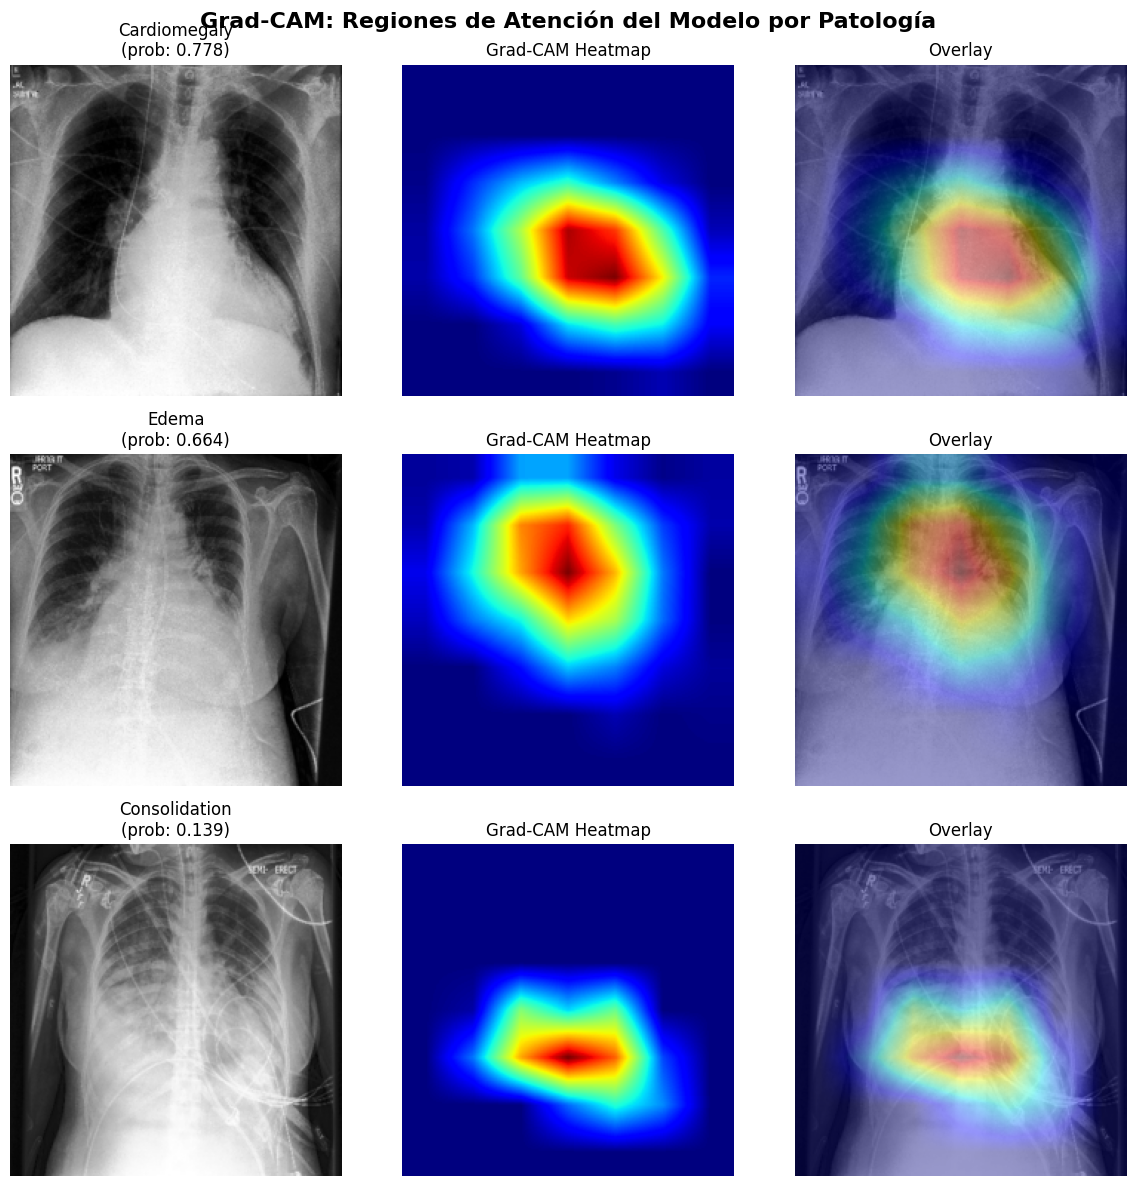
\includegraphics[width=\columnwidth]{figures/gradcam-cardiomegaly-edema-consolidation.png}
    \caption{Grad-CAM: Cardiomegaly (silueta card\'iaca), Edema (campos pulmonares) y Consolidation (opacidad focal). No se detect\'o shortcut learning.}
    \label{fig:gradcam1}
\end{figure}

\begin{figure}[H]
    \centering
    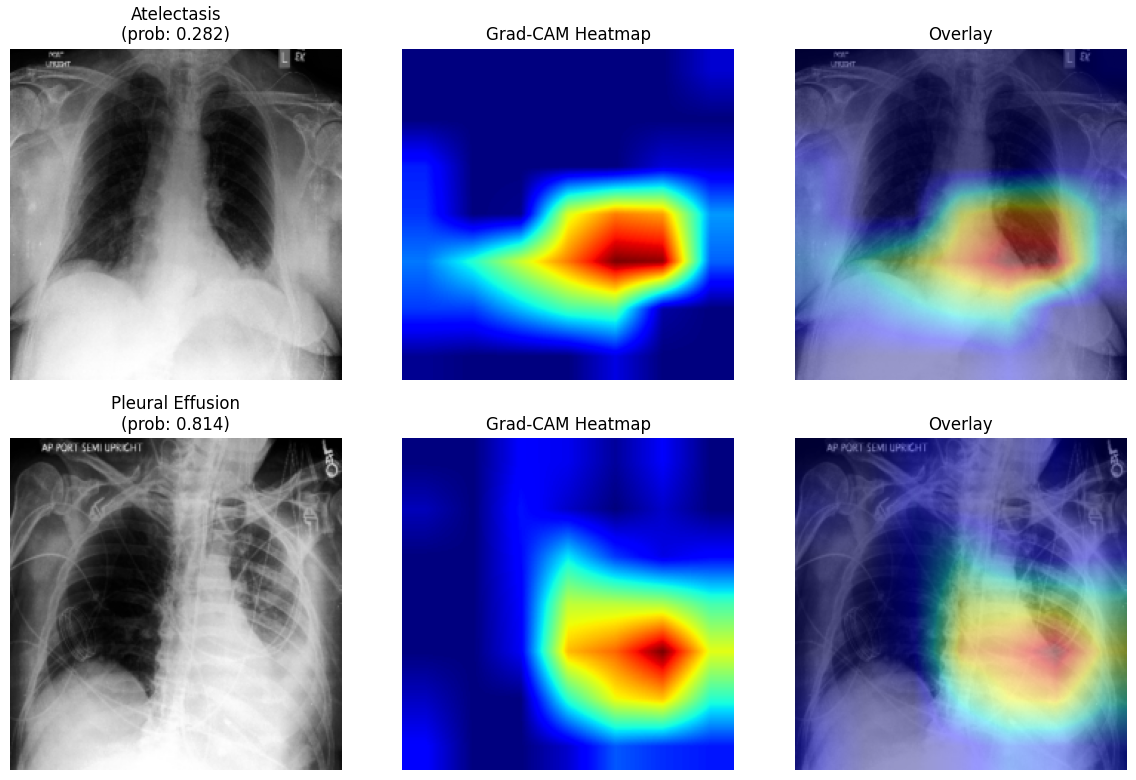
\includegraphics[width=\columnwidth]{figures/gradcam-atelectasis-pleural-effusion.png}
    \caption{Grad-CAM: Atelectasis (base pulmonar) y Pleural Effusion (\'angulos costofr\'enicos). Atenci\'on anat\'omicamente correcta en todas las patolog\'ias.}
    \label{fig:gradcam2}
\end{figure}

Se reconoce la limitaci\'on documentada por \cite{saporta2022benchmarking}: los m\'etodos de saliency son significativamente peores que radi\'ologos en localizaci\'on, por lo que Grad-CAM se utiliza como verificaci\'on de shortcut learning, no como auditor\'ia cl\'inica definitiva.

\subsection{Calibraci\'on}

Se aplic\'o temperature scaling post-hoc sobre el conjunto de validaci\'on, optimizando el par\'ametro $T$ para minimizar el Negative Log-Likelihood. El Error de Calibraci\'on Esperado (ECE) mejor\'o tras la calibraci\'on, confirmando que el modelo requiere ajuste post-hoc para que las probabilidades sean confiables en producci\'on.

\subsection{Hallazgos principales}

\begin{figure}[H]
    \centering
    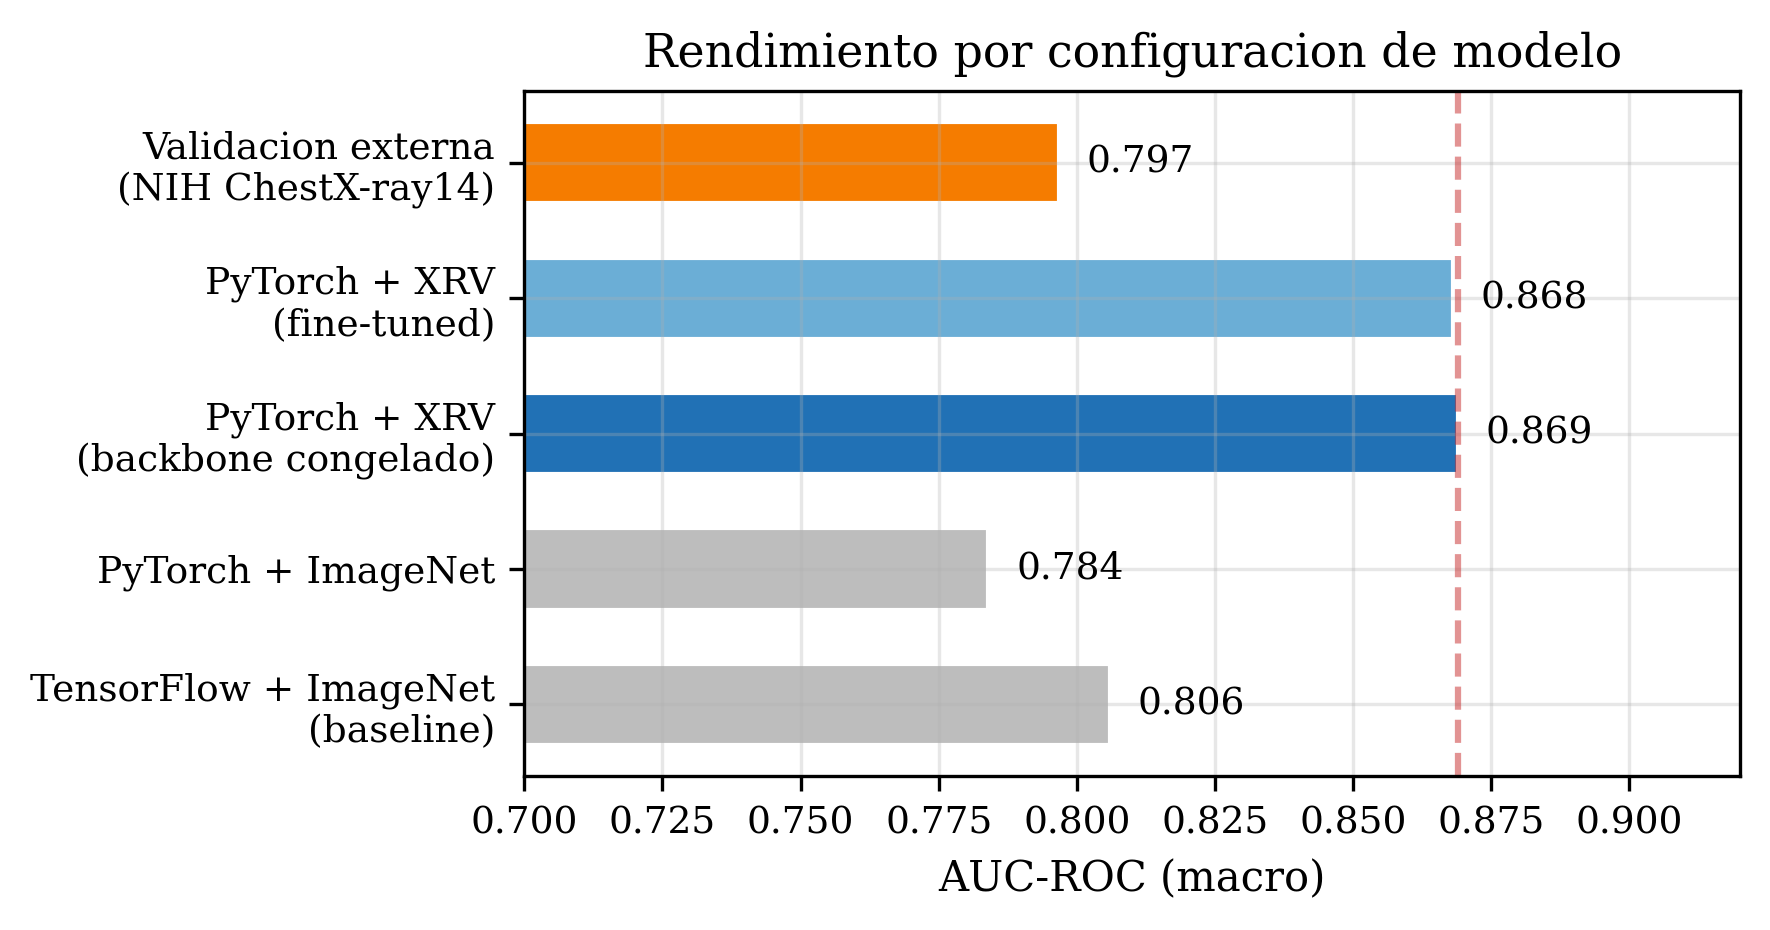
\includegraphics[width=\columnwidth]{figures/auc-roc-model-configs.png}
    \caption{Curvas AUC-ROC por patolog\'ia para la mejor configuraci\'on del modelo (PyTorch + TorchXRayVision, backbone congelado).}
    \label{fig:auc-roc}
\end{figure}

\begin{enumerate}
    \item \textbf{Transfer learning especializado supera al gen\'erico}: TorchXRayVision (preentrenado en radiograf\'ias) supera a ImageNet por 8.4\% AUC. El conocimiento de dominio es cr\'itico.
    \item \textbf{Fine-tuning no mejor\'o}: el backbone XRV ya tiene features \'optimas para las 5 patolog\'ias. El modelo congelado es preferible (m\'as simple, mismo rendimiento).
    \item \textbf{Generalizaci\'on moderada}: 7.2\% de ca\'ida en datos externos es aceptable para screening, pero Atelectasis requiere adaptaci\'on espec\'ifica.
    \item \textbf{Atenci\'on anat\'omica correcta}: Grad-CAM descarta shortcut learning.
    \item \textbf{Sesgo de g\'enero detectado}: gap de 9.2\% en Atelectasis entre pacientes masculinos y femeninos (Secci\'on~\ref{sec:ethics}).
    \item \textbf{Impacto operativo}: inferencia en $\sim$20ms v\'ia ONNX Runtime, compatible con flujo cl\'inico en tiempo real. Modelo autocontenido (normalizaci\'on embebida) que elimina training-serving skew.
\end{enumerate}
